\documentclass[aspectratio=169]{beamer}
% ---- Minimal setup (XeLaTeX) ----
\usepackage{fontspec}
\defaultfontfeatures{Ligatures=TeX}
%\usepackage{luatexja}
%\usepackage{luatexja-fontspec}
%\ltjsetparameter{jacharrange={-9}}
\setmainfont{TeX Gyre Pagella}
\setsansfont{TeX Gyre Heros}
\setmonofont{Inconsolata} % TeX Gyre Cursor} %  Fira Mono}
% Auto-switch by Unicode block
% Font families for non-Latin scripts
\newfontfamily\jafont{Noto Sans CJK JP}
\newfontfamily\krfont{Noto Sans CJK KR}
\newfontfamily\hanfont{Noto Sans CJK SC}
\newfontfamily\devanagarifont{Noto Sans Devanagari}
\newfontfamily\ipafont{Gentium}

% Explicit font-switching macros — use these to wrap non-Latin text
\newcommand{\ja}[1]{{\jafont #1}}          % Japanese
\newcommand{\cn}[1]{{\hanfont #1}}         % Chinese/Mandarin
\newcommand{\ko}[1]{{\krfont #1}}          % Korean
\newcommand{\dv}[1]{{\devanagarifont #1}}  % Devanagari
\newcommand{\ipa}[1]{{\ipafont #1}}        % IPA
\newcommand{\jpf}[1]{\ja{#1}}             % backward-compat alias

% Graceful fallback in PDF bookmarks
\pdfstringdefDisableCommands{%
  \def\ja#1{#1}%
  \def\cn#1{#1}%
  \def\ko#1{#1}%
  \def\dv#1{#1}%
  \def\ipa#1{#1}%
  \def\jpf#1{#1}%
}
% \newfontfamily\emoji{Noto Color Emoji}[Renderer=Harfbuzz,Scale=MatchLowercase]
% \newcommand{\e}[1]{{\emoji #1}}

\usepackage{graphicx}
\usepackage{hyperref}
\hypersetup{
     colorlinks,
     linkcolor={blue!50!black},
     citecolor={red!50!black},
     urlcolor={blue!80!black}
   }
\usepackage{booktabs}
\usepackage{microtype}

\newcommand{\txx}[1]{\textbf{\textcolor{blue}{#1}}}

% --- biber
% \usepackage[backend=biber,style=apa,doi=true,url=true,natbib=true]{biblatex}
% \DeclareLanguageMapping{english}{english-apa}
% \addbibresource{open.bib}
\usepackage[round]{natbib}

% ---- Beamer look ----
\usetheme{Boadilla}
\usecolortheme{seahorse}
\setbeamertemplate{navigation symbols}{}
\setbeamertemplate{itemize items}[circle]
\setbeamertemplate{itemize subitem}[triangle]
%\setbeamertemplate{footline}[frame number]
\setbeamerfont{block body example}{size=\small}
\setbeamerfont{block title example}{size=\small}  % optional: adjust title too
% ---- Section outline slide ----
\AtBeginSection[]{
  \begin{frame}
    \frametitle{Roadmap}
    \small
    \tableofcontents[currentsection, hideothersubsections]%, hideallsubsections]
  \end{frame}
}
\logo{
\includegraphics[width=15mm]{img/UP_logo_FF_horizont_en.png}}

% ---- other packages
\usepackage{tikz}

% ---- Linguistics

\usepackage{langsci-gb4e}
\usepackage{avm}

\usepackage[normalem]{ulem}
\newcommand{\ul}{\uline}
\newcommand{\ull}{\uuline}
\newcommand{\udl}{\dashuline}
\newcommand{\uwl}{\uwave}

\usepackage[e,f,j]{mtg2e}
\newcommand{\cmn}{\mtciteform}
\newcommand{\kor}{\mtciteform}
\renewcommand{\mtcitestyle}[1]{\textcolor{teal}{\textit{#1}}}
\usepackage{xcolor}
 \newcommand{\bs}{\textbackslash}   % backslash
 \newcommand{\cmd}[1]{{\bf \color{red}#1}}   % highlights command
 \newcommand{\wemp}[1]{\ul{#1}}   % highlight
 \newcommand{\emp}[1]{\textbf{\color{blue}{#1}}}   % highlight
 \newcommand{\rel}[1]{\textsc{\color{blue}{#1}}}
 %%% imi zokusei
 \newcommand{\iz}[1]{\textup{\texttt{\color{blue}{\textbf{#1}}}}}
 \newcommand{\con}{\iz}
 \newcommand{\lnk}[1]{\rel{#1}}
 \newcommand{\dff}[1]{\rel{#1}}
\newcommand{\cmp}[1]{{[\textsc{#1}]}}
\newcommand{\elem}[1]{\ensuremath{\langle}\texttt{#1}\ensuremath{\rangle}}
 \newcommand{\lex}[1]{\textbf{\color{teal}{\textit{#1}}}}
 \newcommand{\lng}[1]{\textcolor{teal}{\textit{#1}}}
\newcommand{\wn}[3]{\lex{#1}\ensuremath{_{#2:#3}}}
\usepackage{relsize,xspace}
\newcommand{\wnida}[1]{\asort{\wnid{#1}}}
\newcommand{\wnid}[1]{\textsf{\smaller #1}}
\newcommand{\topic}[1]{\textsc{#1}}
\newcommand{\into}{\ensuremath{\rightarrow}\xspace}
\newcommand{\ent}{\ensuremath{\Rightarrow}\xspace}
\newcommand{\nent}{\ensuremath{\not\Rightarrow}\xspace}
\newcommand{\tot}{\ensuremath{\leftrightarrow}\xspace}

\newcommand{\MyLogo}[1]{}

% \newcommand{\task}{\marginpar{\raisebox{-2ex}{
%       \hspace{-0.5em}\reflectbox{\includegraphics[width=2em]{img/detective.pdf}}}}}
\newcommand{\task}{?}


\setbeamercolor{taskc}{fg=black,bg=red!10}

\newenvironment{taskb}[1][]{%
  \begin{beamercolorbox}[rounded=true,shadow=true,wd=\linewidth,sep=0.5em]{taskc}
    \ifx\relax#1\relax
      % No title - just show content
    \else
      % Title provided
      \textbf{\large ?} #1
      \par\vspace{0.3em}
    \fi
}{%
  \end{beamercolorbox}
  \vspace{0.5em}
}

% \usepackage[T1]{fontenc}
% \usepackage{lmodern}
% \usepackage{microtype}

\usepackage{minted}
\usemintedstyle{emacs}
\setminted{bgcolor=gray!10}

\usepackage{tikz}
\usetikzlibrary{arrows.meta,positioning,fit,calc}

\tikzset{%
  % classes
  avm/.style={draw, rounded corners, align=left, inner sep=4pt},
%  avm/.style={draw, rounded corners, align=center, inner sep=4pt},
  word/.style={avm, fill=green!7},
  sense/.style={avm, fill=blue!7},
  synset/.style={avm, fill=gray!10},
  ili/.style={avm, fill=orange!10},
  % edge styles
  rel/.style={-Latex, thick},
  birel/.style={Latex-Latex, thick},
  weak/.style={-Latex, thick, opacity=0.65},
  biweak/.style={Latex-Latex, thick, opacity=0.65},
  group/.style={draw, rounded corners, inner sep=6pt, dashed},
  box/.style={draw, rounded corners, align=center, inner sep=4pt},
  small/.style={font=\small},
  tiny/.style={font=\tiny},
}%
\newcommand{\avmtype}{\scriptsize\itshape\color{black!70}\raggedright}
%\newcommand{\avmtype}{\scriptsize\itshape\color{black!70}}
\newcommand{\avmcontent}{\small}
\newcommand{\avmnode}[4][]{%
  % #1 = extra TikZ options
  % #2 = class (word | sense | synset | ili ...)
  % #3 = node name
  % #4 = content
  \node[#2, #1] (#3) {%
    {\avmtype #2}\\
    {\avmcontent \shortstack{#4}}%
  };
}

\title{WordNet Structure: Words, Senses, Synsets, and Relations
\\ Manipulating wordnets with \texttt{wn}}
\author{Francis Bond}
\date{\today}
% ============================




\begin{document}

% ------------------------------------------------------------
\begin{frame}
  \titlepage
\end{frame}

% ------------------------------------------------------------
\begin{frame}{Big idea: a lexicon organized by concepts}
\begin{itemize}
  \item A \textbf{word form} can express \textbf{multiple meanings} (polysemy).
  \item A \textbf{meaning} can be expressed by \textbf{multiple word forms} (synonymy).
  \item WordNets model meaning with:
    \begin{itemize}
      \item \textbf{Words} (forms)
      \item \textbf{Senses} (a word-in-a-particular-meaning)
      \item \textbf{Synsets} (concepts; sets of near-synonymous senses)
      \item \textbf{Relations} between synsets/senses
    \end{itemize}
\end{itemize}
\end{frame}



% ------------------------------------------------------------
\begin{frame}{Words $\rightarrow$ Senses $\rightarrow$ Synsets}
\centering
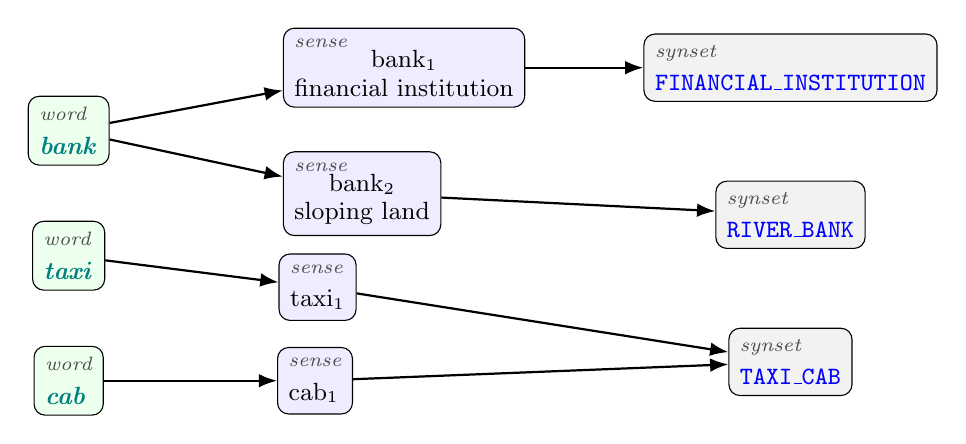
\begin{tikzpicture}[node distance=10mm]
  % Words
  \avmnode{word}{wbank}{\lex{bank}};
  \avmnode[below=7mm of wbank]{word}{wtaxi}{\lex{taxi}};
  \avmnode[below=7mm of wtaxi]{word}{wcab}{\lex{cab}};

  % Senses
  \avmnode[right=22mm of wbank, yshift=8mm]{sense}{sbank1}{bank\textsubscript{1}\\  financial institution};
  \avmnode[right=22mm of wbank, yshift=-8mm]{sense}{sbank2}{bank\textsubscript{2}\\ sloping land};
  \avmnode[right=22mm of wtaxi, yshift=-4mm]{sense}{staxi1}{taxi\textsubscript{1}};
  \avmnode[right=22mm of wcab]{sense}{scab1}{cab\textsubscript{1}};

  % Synsets
  \avmnode[right=15mm of sbank1]{synset}{synfin}{\iz{FINANCIAL\_INSTITUTION}};
  \avmnode[below=10mm of synfin]{synset}{synriver}{\iz{RIVER\_BANK}};
  \avmnode[below=10mm of synriver]{synset}{syntaxi}{\iz{TAXI\_CAB}};

  % Links
  \draw[rel] (wbank) -- (sbank1);
  \draw[rel] (wbank) -- (sbank2);
  \draw[rel] (wtaxi) -- (staxi1);
  \draw[rel] (wcab) -- (scab1);

  \draw[rel] (sbank1) -- (synfin);
  \draw[rel] (sbank2) -- (synriver);
  \draw[rel] (staxi1) -- (syntaxi);
  \draw[rel] (scab1) -- (syntaxi);

  % Labels
  % \node[tiny, above=1mm of synfin] {concept node};
  % \node[tiny, above=1mm of sbank1] {disambiguation unit};
\end{tikzpicture}

\vspace{2mm}
\small
Key:  \textbf{senses} link \textbf{words} to \textbf{synsets} (concepts).
\end{frame}



\begin{frame}{What \textbf{lexicons} have}

\begin{itemize}
\item A lexicon is a collection of synsets, senses, words and relations for a given language
\item It will normally have some metadata associated with it
  \begin{itemize}
  \item Label
  \item License
  \item Language
  \end{itemize}
\item The \texttt{wn} module has a collection of wordnets you can download easily
\item If you have a wordnet in the LMF format, you can load it locally
\end{itemize}
\end{frame}


\begin{frame}[fragile]{Loading and describing a lexicon in WN}
\begin{minted}{python}
>>> import wn
>>> wn.download('omw-en:1.4')
>>> ewn = wn.Wordnet('omw-en:1.4')
>>> print(ewn.describe())
Primary lexicons:
  omw-en:1.4
    Label  : OMW English Wordnet based on WordNet 3.0
    URL    : None
    License: https://wordnet.princeton.edu/license-and-commercial-use
    Words  : 156584 (a: 21538, n: 119034, r: 4481, v: 11531)
    Senses : 206978
    Synsets: 117659 (a: 7463, n: 82115, r: 3621, s: 10693, v: 13767)
    ILIs   : 117659
>>> wn.projects() # gives a list of downloadable wordnets
... 
\end{minted}
\end{frame}


\begin{frame}[fragile]{Adding, removing and listing lexicons with WN}
\begin{minted}{python}
>>> wn.add('path/to/omw-nb:1.4.xz')
>>> wn.remove('omw-nb:1.4')
>>> for lex in wn.lexicons():
...     print(f'{lex.id}:{lex.version}\t{lex.label}')
...
omw-en:1.4      OMW English Wordnet based on WordNet 3.0
omw-nb:1.4      Norwegian Wordnet (Bokmål)
odenet:1.3      Offenes Deutsches WordNet
ewn:2020        English WordNet
...
\end{minted}
\end{frame}


% ============================================================
% NEW SLIDE 1: Word-only properties
% ============================================================
\begin{frame}{What  \textbf{Words} have}
\begin{itemize}
  \item \textbf{Canonical Form (Lemma)}: the written form(s) used in the lexicon
  \item \textbf{Part of speech}
  \item \textbf{Variant forms}
    \begin{itemize}
    \item spelling variants (\eng{colour/color}), scripts (\jpn{\ja{犬 / いぬ}}), casing/diacritics policy,
      irregular forms  (\eng{child/children} [pl]), 
    \end{itemize}
  \item \textbf{Form metadata} (when present in a resource)
    \begin{itemize}
      \item pronunciations, transliterations, orthographic variants type (US/UK)
      \item morphological class (plural, past), if the resource encodes them at word-level
    \end{itemize}
  \item \textbf{Derivations:} links to words related by derivation 
  \item \textbf{Sense(s)}:
    \begin{itemize}
      \item one \texttt{Word} can have multiple \texttt{Sense}s (polysemy)
      \item all those senses share the same \emph{string forms} but differ in meaning
    \end{itemize}
\end{itemize}

% \smallskip
% \centering
% \begin{tikzpicture}[node distance=10mm]
%   \node[word] (w) {Word\\\textbf{bank}};
%   \node[box, right=18mm of w] (forms) {word-level\\properties\\\tiny lemma, forms,\\tiny variants, pron.};
%   \draw[rel] (w) -- (forms);
% \end{tikzpicture}
\end{frame}

\begin{frame}[fragile]{Form metadata example}
\begin{minted}{python}
<LexicalEntry id="ex-gato-n">
    <Lemma writtenForm="gato" partOfSpeech="n">
      <Tag category="gender">masculine</Tag>
    </Lemma>
    <Form writtenForm="gatos">
        <Tag category="number">plural</Tag>
    </Form>
</LexicalEntry>
\end{minted}
  \begin{itemize}
  \item Grammatical properties such as gender, number, case, and tense can be represented with the \elem{Tag} element.
  \item The \elem{Tag} element has a category attribute which indicates the type of grammatical property, and the value is the text of the tag
  \item  A universal tagging scheme is not prescribed --- wordnet project owners are free to choose a scheme 

\end{itemize}
  
\end{frame}

\begin{frame}[fragile]{Finding Words in WN}
\begin{minted}{python}
>>> wn.words('pencil')
[Word('ewn-pencil-n'), Word('ewn-pencil-v')]
>>> wn.words('pencil', pos='v')
[Word('ewn-pencil-v')]
len(wn.words())
311711
>>> len(wn.words(pos='v'))
29419
>>> len(wn.words(pos='v', lexicon='ewn'))
11595
>>> wn.word('ewn-pencil-n', lexicon='ewn')
Word('ewn-pencil-n')
\end{minted}
\end{frame}

\begin{frame}[fragile]{Exploring Words in WN}
\begin{minted}{python}
>>> w = wn.words('goose')[0]
>>> w.pos  # part of speech
'n'
>>> w.forms()  # other word forms (e.g., irregular inflections)
['goose', 'geese']
>>> w.lemma()  # canonical form
'goose'
>>> w.derived_words()
[Word('ewn-gosling-n'), Word('ewn-goosy-s'), Word('ewn-goosey-s')]
>>> w.senses()
[Sense('ewn-goose-n-01858313-01'), Sense('ewn-goose-n-10177319-06'), Sense('ewn-goose-n-07662430-01')]
>>> w.synsets()
[Synset('ewn-01858313-n'), Synset('ewn-10177319-n'), Synset('ewn-07662430-n')]
>>> w.forms()[0].pronunciations()[0].value  # in oewn 
"'gu:s"
\end{minted}
%"ˈɡuːs"
\end{frame}



% ============================================================
% NEW SLIDE 2: Sense-only properties
% ============================================================
\begin{frame}{What \textbf{Senses} have}
\begin{itemize}
  \item A \textbf{sense} is the pairing: \textbf{Word} $\times$ \textbf{Synset}
  \item Sense-level properties often include:
    \begin{itemize}
      \item \textbf{Sense IDs / keys} (resource-specific identifiers)
      \item \textbf{Frequency / counts} (e.g., corpus-based tagging counts)
      \item \textbf{Derivations} (constrained by meaning)
      \item \textbf{Usage examples} (example sentences tied to this meaning)
      \item \textbf{Syntactic/verb frames} (common in some WordNet-style resources)
      \item \textbf{Sense-level relations} such as antonymy
    \end{itemize}
  \item Why sense-level? Because \textbf{frequency and examples depend on the meaning}, not just the string or the concept.
\end{itemize}

% \smallskip
% \centering
% \begin{tikzpicture}[node distance=10mm, scale=0.88, transform shape]
%   \node[word] (w) {Word\\\textbf{bank}};
%   \node[synset, right=48mm of w] (syn) {Synset\\\textbf{FINANCIAL\_INSTITUTION}};
%   \node[sense, above=0mm of $(w)!0.5!(syn)$] (s) {Sense\\bank\textsubscript{1}};
%   \draw[rel] (w) -- (s);
%   \draw[rel] (s) -- (syn);

%   \node[box, below=8mm of s, font=\scriptsize] (props)
%     {sense-only\\properties\\\tiny frequency, examples,\\\tiny sense key, frames};
%   \draw[rel] (s) -- (props);
% \end{tikzpicture}

% \begin{tikzpicture}[node distance=10mm]
%   \node[word] (w) {Word\\\textbf{bank}};
%   \node[synset, right=44mm of w] (syn) {Synset\\\textbf{FINANCIAL\_INSTITUTION}};
%   \node[sense, above=0mm of $(w)!0.5!(syn)$] (s) {Sense\\bank\textsubscript{1}};
%   \draw[rel] (w) -- (s);
%   \draw[rel] (s) -- (syn);

%   \node[box, below=12mm of s] (props) {sense-only\\properties\\\tiny frequency, examples,\\tiny sense key, frames};
%   \draw[rel] (s) -- (props);
% \end{tikzpicture}
\end{frame}


\begin{frame}[fragile]{Finding Senses in WN}
\begin{minted}{python}
>>> ewn.senses('plow', pos='n')
[Sense('ewn-plow-n-03973894-01')]
>>> ewn.sense('ewn-plow-v-01745745-01')
Sense('ewn-plow-v-01745745-01')
>>> len(ewn.senses(pos='n'))
146347
\end{minted}
\end{frame}

\begin{frame}[fragile]{Exploring Senses in WN}
\begin{minted}{python}
>>> s = ewn.senses('dark', pos='n')[0]
>>> s.word()    # each sense links to a single word
Word('ewn-dark-n')
>>> s.synset()  # each sense links to a single synset
Synset('ewn-14007000-n')
>>> s.get_related('antonym')
[Sense('ewn-light-n-14006789-01')]
>>> s.get_related('derivation')
[Sense('ewn-dark-a-00273948-01')]
>>> s.metadata()  # omw-en:1.4
{'identifier': 'dark%1:26:00::'}
>>> s.counts()
[2]
>>> ewn.senses('darken', pos='v')[0].frames()
['Something ----s']
\end{minted}
% >>> ewn.senses('darken', pos='v')[1].frames()
% ['Something ----s something']
\end{frame}

% ============================================================
% NEW SLIDE 3: Synset-only properties (ILI, lexicographer files)
% ============================================================
\begin{frame}{What \textbf{Synsets} have}
\begin{itemize}
  \item A \textbf{synset} represents a \textbf{concept} (language-internal, but linkable).
  \item Typical synset-level properties:
    \begin{itemize}
    \item \textbf{Definition / gloss} (concept description)
    \item \textbf{Usage examples} (example sentences)
      
    \item \textbf{Part of speech} (noun/verb/adj/adv in many resources)
    \item \textbf{Semantic fields / domains} (e.g., \emph{lexicographer files})
    \item \textbf{Concept relations}: hypernym, meronym, cause, etc.
    \item \textbf{ILI links} (interlingual index), when available
    \end{itemize}
  \item Why synset-level? Because these describe the \textbf{concept itself}, independent of which word expresses it.
\end{itemize}

% \smallskip
% \centering
% \begin{tikzpicture}[node distance=9mm]
%   \node[synset] (syn) {Synset\\\textbf{DOG}};
%   \node[ili, right=18mm of syn] (ili) {ILI\\\textbf{i123456}};
%   \node[box, above=10mm of syn] (gloss) {synset-level\\properties\\\tiny gloss, domain,\\tiny lexfile, POS};
%   \node[synset, below=12mm of syn] (hyper) {Synset\\\textbf{CANINE}};

%   \draw[rel] (syn) -- node[above, tiny] {ili} (ili);
%   \draw[rel] (syn) -- node[left, tiny] {hypernym} (hyper);
%   \draw[rel] (syn) -- (gloss);
% \end{tikzpicture}
\end{frame}


\begin{frame}[fragile]{Finding Synsets in WN}
\begin{minted}{python}
>>> wn.synsets('scepter')
[Synset('ewn-14467142-n'), Synset('ewn-07282278-n')]
>>> wn.synset('ewn-07282278-n').ili
'i74874'
>>> wn.synsets(ili='i74874')
[Synset('ewn-07282278-n'), Synset('wnja-07267573-n'), Synset('frawn-07267573-n')]
\end{minted}
\end{frame}

\begin{frame}[fragile, allowframebreaks]{Exploring Synsets in WN}
\begin{minted}{python}
>>> ss = wn.synsets('hound', pos='n')[0]
>>> ss.senses()
[Sense('ewn-hound-n-02090203-01'), Sense('ewn-hound_dog-n-02090203-02')]
>>> ss.words()
[Word('ewn-hound-n'), Word('ewn-hound_dog-n')]
>>> ss.lemmas()
['hound', 'hound dog']
>>> ss.definition()
'any of several breeds of dog used for hunting typically having large drooping ears'
\end{minted}
\framebreak
\begin{minted}{python}
>>> ss.hypernyms()
[Synset('ewn-02089774-n')]
>>> ss.hypernyms()[0].lemmas()
['hunting dog']
>>> len(ss.hyponyms())
20
>>> ss.hyponyms()[0].lemmas()
['Afghan', 'Afghan hound']
>>> ss.max_depth()
15
>>> ss.shortest_path(wn.synsets('dog', pos='n')[0])
[Synset('ewn-02090203-n'), Synset('ewn-02089774-n'), Synset('ewn-02086723-n')]
\end{minted}
\end{frame}







% ============================================================
% ADD THIS SLIDE: POS-specific synsets with multiple member senses
% ============================================================
\begin{frame}{POS-specific variants: concepts live in POS-specific synsets}
\small
\begin{itemize}
  \item A synset is typically \textbf{POS-specific} (noun synset vs adjective synset, etc.).
  \item The “same general idea” across POS is modeled via \textbf{relations between synsets},
        not by mixing POS inside one synset.
\end{itemize}

\centering
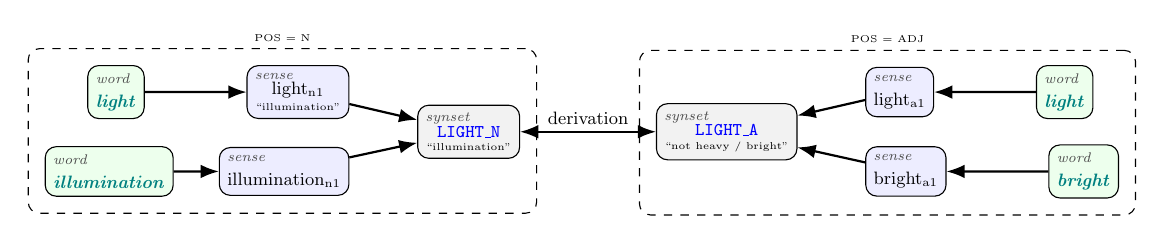
\begin{tikzpicture}[node distance=8mm, scale=0.72, transform shape]
  % Noun side
  \avmnode{synset}{syn_n}{\iz{LIGHT\_N}\\\tiny “illumination”};
  \avmnode[left=12mm of syn_n, yshift=7mm]{sense}{s_n1}{light\textsubscript{n1}\\\tiny “illumination”};
  \avmnode[left=12mm of syn_n, yshift=-7mm]{sense}{s_n2}{illumination\textsubscript{n1}};
  \avmnode[left=18mm of s_n1]{word}{w_light_n}{\lex{light}};
  \avmnode[left=8mm of s_n2]{word}{w_illum}{\lex{illumination}};

  % Adjective side
  \avmnode[right=24mm of syn_n]{synset}{syn_a}{\iz{LIGHT\_A}\\\tiny “not heavy / bright”};
  \avmnode[right=12mm of syn_a, yshift=7mm]{sense}{s_a1}{light\textsubscript{a1}};
  \avmnode[right=12mm of syn_a, yshift=-7mm]{sense}{s_a2}{bright\textsubscript{a1}};
  \avmnode[right=18mm of s_a1]{word}{w_light_a}{\lex{light}};
  \avmnode[right=18mm of s_a2]{word}{w_bright}{\lex{bright}};

  % Membership
  \draw[rel] (w_light_n) -- (s_n1);
  \draw[rel] (w_illum) -- (s_n2);
  \draw[rel] (s_n1) -- (syn_n);
  \draw[rel] (s_n2) -- (syn_n);

  \draw[rel] (w_light_a) -- (s_a1);
  \draw[rel] (w_bright) -- (s_a2);
  \draw[rel] (s_a1) -- (syn_a);
  \draw[rel] (s_a2) -- (syn_a);

  % Cross-POS relation
  \draw[birel] (syn_n) -- node[font=\small, above] {derivation} (syn_a);

  % Grouping
  \node[group, fit=(w_illum)(s_n2)(syn_n)(s_n1), label={[font=\tiny]above:POS = N}] {};
  \node[group, fit=(syn_a)(w_bright)(s_a2)(s_a1), label={[font=\tiny]above:POS = ADJ}] {};
\end{tikzpicture}


\end{frame}


% ============================================================
% NEW SLIDE 4: Cheat-sheet diagram (where does info live?)
% ============================================================
\begin{frame}{Cheat sheet: where does each kind of information live?}
\centering
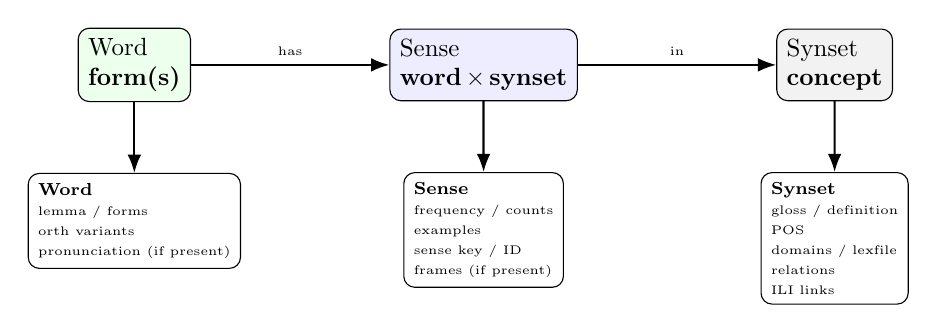
\begin{tikzpicture}[node distance=9mm, scale=0.90, transform shape]
  \node[word] (w) {Word\\\textbf{form(s)}};
  \node[sense, right=28mm of w] (s) {Sense\\\textbf{word}\,$\times$\,\textbf{synset}};
  \node[synset, right=28mm of s] (y) {Synset\\\textbf{concept}};

  \draw[rel] (w) -- node[font=\tiny, above] {has} (s);
  \draw[rel] (s) -- node[font=\tiny, above] {in} (y);

  \node[box, below=10mm of w, align=left, font=\scriptsize] (wprops)
    {\textbf{Word}\\\tiny lemma / forms\\\tiny orth variants\\\tiny pronunciation (if present)};
  \node[box, below=10mm of s, align=left, font=\scriptsize] (sprops)
    {\textbf{Sense}\\\tiny frequency / counts\\\tiny examples\\\tiny sense key / ID\\\tiny frames (if present)};
  \node[box, below=10mm of y, align=left, font=\scriptsize] (yprops)
    {\textbf{Synset}\\\tiny gloss / definition\\\tiny POS\\\tiny domains / lexfile\\\tiny relations\\\tiny ILI links};

  \draw[rel] (w) -- (wprops);
  \draw[rel] (s) -- (sprops);
  \draw[rel] (y) -- (yprops);
\end{tikzpicture}

\vspace{2mm}
\scriptsize
Rule of thumb: \emph{form} $\rightarrow$ Word;\quad \emph{usage of a meaning} $\rightarrow$ Sense;\quad \emph{concept + relations} $\rightarrow$ Synset.
\end{frame}

% ------------------------------------------------------------
\begin{frame}{Relations: building a graph over concepts}
\centering
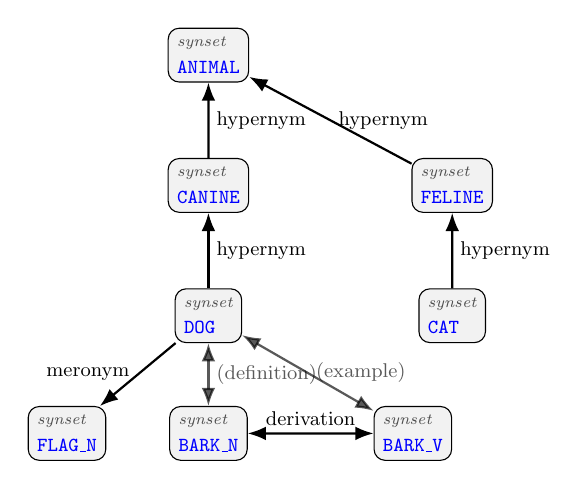
\begin{tikzpicture}[node distance=10mm, scale=0.80, transform shape]
  \avmnode{synset}{dog}{\iz{DOG}};
  \avmnode[above=12mm of dog]{synset}{canine}{\iz{CANINE}};
  \avmnode[above=12mm of canine]{synset}{animal}{\iz{ANIMAL}};

  \avmnode[right=28mm of dog]{synset}{cat}{\iz{CAT}};
  \avmnode[above=12mm of cat]{synset}{feline}{\iz{FELINE}};


  \avmnode[below=10mm of dog]{synset}{bark}{\iz{BARK\_N}};
  \avmnode[left=10mm of bark]{synset}{flag}{\iz{FLAG\_N}};
  \avmnode[right=20mm of bark]{synset}{barkv}{\iz{BARK\_V}};

  \draw[rel] (dog) -- node[font=\small, right]{hypernym} (canine);
  \draw[rel] (canine) -- node[font=\small, right]{hypernym} (animal);
  \draw[rel] (cat) -- node[font=\small, right]{hypernym} (feline);
  \draw[rel] (feline) -- node[font=\small, right]{hypernym} (animal);

%  \draw[weak] (dog) -- node[font=\small, above] {related} (cat);
  \draw[rel] (dog) -- node[font=\small, left] {meronym} (flag);
  \draw[biweak] (dog) -- node[font=\small, right] {(definition)} (bark);
  \draw[biweak] (dog) -- node[font=\small, right] {(example)} (barkv);
  \draw[birel] (barkv) -- node[font=\small, above] {derivation} (bark);


\end{tikzpicture}

\smallskip
\small
WordNets are \textbf{graphs}: taxonomy-like relations (e.g.\ hypernymy) plus many non-taxonomic links (meronymy, cause, related, used in example/definition etc.).
\end{frame}

% ------------------------------------------------------------
\begin{frame}{The taxonomy: a (mostly) rooted hierarchy for nouns}
\centering
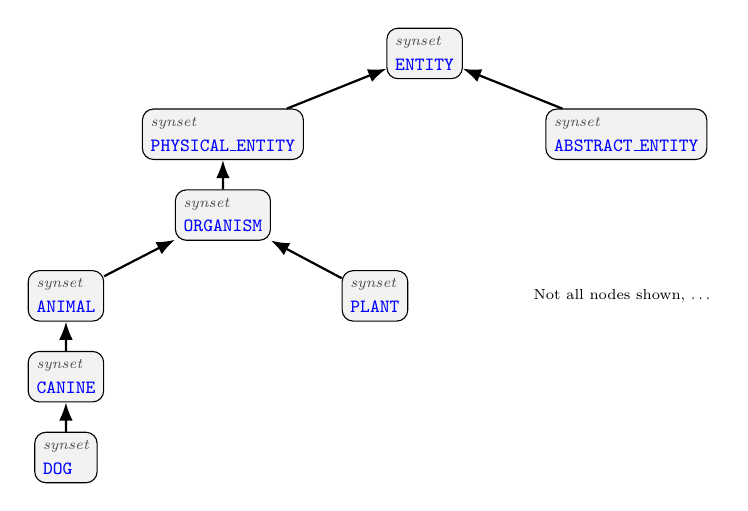
\begin{tikzpicture}[node distance=8mm, scale=0.75, transform shape, xshift=-6mm]
  \avmnode{synset}{entity}{\iz{ENTITY}};
  \avmnode[below left=5mm and 14mm of entity]{synset}{physical}{\iz{PHYSICAL\_ENTITY}};
  \avmnode[below right=5mm and 14mm of entity]{synset}{abstract}{\iz{ABSTRACT\_ENTITY}};
          [
  \avmnode[below=5mm of physical]{synset}{organism}{\iz{ORGANISM}};
  \avmnode[below left=5mm and 12mm of organism]{synset}{animal}{\iz{ANIMAL}};
  \avmnode[below right=5mm and 12mm of organism]{synset}{plant}{\iz{PLANT}};
          [
  \avmnode[below=5mm of animal]{synset}{canine}{\iz{CANINE}};
  \avmnode[below=5mm of canine]{synset}{dog}{\iz{DOG}};

  \draw[rel] (physical) -- (entity);
  \draw[rel] (abstract) -- (entity);
  \draw[rel] (organism) -- (physical);
  \draw[rel] (animal) -- (organism);
  \draw[rel] (plant) -- (organism);
  \draw[rel] (canine) -- (animal);
  \draw[rel] (dog) -- (canine);



  \node[font=\scriptsize, align=left, right=20mm of plant]
    {Not all nodes shown, \ldots};
  
\end{tikzpicture}

Multiple inheritance is possible, loops are not, for OEWN 2025, verbs are also rooted.
\end{frame}

% ------------------------------------------------------------
\begin{frame}{Lexicons, IDs, and versions (in \texttt{wn})}
\begin{itemize}
  \item A \textbf{WordNet resource} is packaged as a \textbf{lexicon} (often: 1 lexicon per resource).
  \item \texttt{wn} supports multiple lexicons (and multiple versions) in one database.
  \item Lexicon specifiers (examples):
    \begin{itemize}
      \item \texttt{ewn:2020} = a specific lexicon \& version
      \item \texttt{ewn:*} = all versions of \texttt{ewn}
      \item \texttt{*} = all lexicons
    \end{itemize}
\end{itemize}

\vspace{2mm}
\small
Most of the time it is better to use a single lexicon (e.g. \texttt{ewn=wn.Wordnet('oewn:2024')})
\end{frame}

% ------------------------------------------------------------
\begin{frame}{Interlingual Index (ILI): linking concepts across languages}
\centering
\begin{tikzpicture}[node distance=10mm]
  % Language synsets
  \avmnode{synset}{en_dog}{EN \iz{DOG}};
  \avmnode[below=10mm of en_dog]{synset}{de_hund}{DE \iz{HUND}};
  \avmnode[below=10mm of de_hund]{synset}{ja_inu}{JA \iz{\ja{犬}} (inu)};

  % ILI
  \avmnode[right=30mm of de_hund]{ili}{ili_dog}{\iz{i46360}};

  % Links
  \draw[rel] (en_dog) -- node[above, tiny] {ili} (ili_dog);
  \draw[rel] (de_hund) -- node[above, tiny] {ili} (ili_dog);
  \draw[rel] (ja_inu) -- node[below, tiny] {ili} (ili_dog);

  % Explanation box
  \node[group, fit=(en_dog)(ja_inu), label={[tiny]above:language-specific synsets}] {};
  \node[group, fit=(ili_dog), label={[tiny]above:interlingual pivot}] {};

\end{tikzpicture}

\smallskip
\small
ILI enables “same concept, different languages” queries when lexicons provide ILI links.
\end{frame}


\begin{frame}{Using the ILI} 

  \begin{itemize}
  \item Wordnets linked to the ILI can be connected
  \item Concepts with the same ILI should be the same across all languages
  \item So we would expect them to be translation equivalents
  \item If one language has a synset with an ILI and another doesn't then this should indicate a lexical gap.
    \begin{itemize}
    \item Although sometimes it just means that the concept has not been added yet
    \end{itemize}
  \item A synset can be marked as \texttt{Lexicalized=False}  (default \texttt{True})
    \begin{itemize}
    \item This means that it has no native word
    \item If it has senses, then they are compositional phrases (like \ja{雌虎} \jpn[female tiger]{mesu.tora} for \eng{tigress})
    \item Very few wordnets have this implemented (they were introduced by the Multiwordnet project)
    \end{itemize}
  \end{itemize}
  
\end{frame}

\begin{frame}[fragile]{Translating using the ILI}

\begin{minted}{python}
# translating  a word gives a list of senses
>>> for sense, ja_words in w.translate(lang='ja').items():  
...     print(sense, ja_words)
...
Sense('ewn-goose-n-01858313-01') [Word('wnja-n-1254'), Word('wnja-n-33090'), Word('wnja-n-38995')]
Sense('ewn-goose-n-10177319-06') []
Sense('ewn-goose-n-07662430-01') [Word('wnja-n-1254')]
# Translating a sense gives a more focused list of senses
>>> s.translate(lang='fr') 
[Sense('frawn-lex52992--13983515-n')]
>>> s.translate(lang='fr')[0].word().lemma()
'obscurité'
# Translating a synset gives a list of synsets (but normally just one)
>>> ss.translate(lang='fr')  # translation returns a list of synsets
[Synset('frawn-02087551-n')]
\end{minted}
% >>> ss.translate(lang='fr')[0].lemmas()
% ['chien', 'chien de chasse']
\end{frame}

% ------------------------------------------------------------
% \begin{frame}{How this maps to the \texttt{wn} Python model}
% \centering
% \begin{tikzpicture}[node distance=10mm]
%   \node[box] (Word) {\texttt{Word}};
%   \node[box, right=18mm of Word] (Sense) {\texttt{Sense}};
%   \node[box, right=18mm of Sense] (Synset) {\texttt{Synset}};
%   \node[box, above=12mm of Synset] (Lexicon) {\texttt{Lexicon}};

%   \draw[rel] (Word) -- node[above, tiny] {\texttt{.senses()}} (Sense);
%   \draw[rel] (Sense) -- node[above, tiny] {\texttt{.synset()}} (Synset);
%   \draw[rel] (Synset) -- node[right, tiny] {belongs to} (Lexicon);

%   \node[box, below=14mm of Synset] (Rel) {\texttt{SynsetRelation}};
%   \draw[rel] (Synset) -- node[left, tiny] {\texttt{.relations()}} (Rel);
%   \draw[rel] (Rel) -| node[below, tiny] {targets} (Synset);

%   \node[small, align=left, below=18mm of Word] {
%   Typical workflow: \texttt{wn.words()} $\rightarrow$ \texttt{Word.senses()} $\rightarrow$ \texttt{Sense.synset()}\\
%   then traverse: \texttt{Synset.relations()} (or taxonomy helpers).
%   };

% \end{tikzpicture}
% \end{frame}


\begin{frame}[fragile]{Some other useful functionality}

  \begin{itemize}
  \item You can set the directory where \texttt{wn}'s data is stored.
\begin{minted}{python}
>>> wn.config.data_directory = ".cache/wn"
\end{minted}
    This is useful to keep the db small and focused
  \item You can use \texttt{wn} to validate a wordnet
\begin{minted}{bash}
$ python -m wn validate english-wordnet-2021.xml --output-file errors.json
\end{minted}
  \item There is a whole \href{https://wn.readthedocs.io/en/latest/cli.html}{command line interface}
where you can list projects (downloadable), lexicons (downloaded), load lexicons
 and more
  \end{itemize}
  
\end{frame}


% ------------------------------------------------------------
\begin{frame}{Summary: what to remember}
\begin{enumerate}
  \item \textbf{Synset $\approx$ concept node}; a set of synonyms, that makes up a concept. Can be non-lexicalized!
  \item \textbf{Relations} turn synsets and senses into a richly typed graph.
  \item \textbf{Taxonomy} (hypernymy) gives a hierarchy (esp.\ nouns).
  \item \textbf{Lexicons} + versions allow reproducibility.
  \item \textbf{ILI} enables cross-lingual alignment when available.
  \item \textbf{Properties live at different layers}: form (Word), usage (Sense), concept (Synset).
  \end{enumerate}
  
Different Wordnet Projects contain different information, OMW tries to harmonize when possible

\end{frame}



\end{document}
%%% Local Variables: 
%%% coding: utf-8
%%% mode: latex
%%% TeX-PDF-mode: t
%%% TeX-engine: xetex
%%% TeX-command-extra-options: "--shell-escape"
%%% End: 
